\section{Licencias}
\frame
{
	\frametitle{Licencias}
	\begin{center}
	Licencias
	\end{center}
}

\subsection{Que son las licencias?}
\frame
{

	\frametitle{Licencias}
	\begin{itemize}
	\item Una \textbf{Licencia de software} (en ingles software license) es la autorizacion o permiso concedida por el titular del derecho de autor, en cualquier forma contractual, al usuario de un programa informatico, para utilizar este en una forma determinada y de conformidad con unas condiciones convenidas.La licencia, que puede ser gratuita u onerosa, precisa los derechos (de uso, modificaci�n y/o redistribucion) concedidos a la persona autorizada y sus limites. Ademas, puede se�alar el plazo de duraci�n, el territorio de aplicacion y todas las demas cl�usulas que el titular del derecho de autor establezca.
	\end{itemize}

}

\subsection{Tipos Licencias}
\frame
{
	\frametitle{Tipos}
	\begin{itemize}
	\item \textbf{Derechos que cada autor}
		\begin{itemize}
		\item \textbf{Licencia de software libre sin protecci�n heredada}
			\begin{itemize}
			\item Se puede crear una obra derivada sin que esta tenga obligaci�n de protecci�n alguna. Muchas licencias pertenecen a esta clase, entre otras:
			\item BSD License.
			\item MIT License.
			\end{itemize}
		
		\item \textbf{Licencia de software libre con protecci�n heredada}
			\begin{itemize}
			\item Licencia irrenunciable, obra derivada protegida.
			\item Artistic License.
			\item Common Public License v.1.0.
			\item GNU General Public License v.2.0.
			\item GNU Lesser General Public License v.2.1.
			\item Mozilla Public License.
			\end{itemize}
			
		\end{itemize}

		
	\item \textbf{Segun su destinatario}
		\begin{itemize}
		\item Licencia de Usuario FinalEn ingl�s EULA o end user license agreement, es una licencia en que se permite s�lo el uso del mismo.
		\end{itemize}
	\end{itemize}
}
\subsection{Clasificacion}
\frame
{
        \frametitle{Clasificacion}
        \begin{itemize}
     	\item Software libre
	\item Software de dominio p�blico.
	\item Software privativo
	\item Freeware.
	\item Shareware.
	\item Software Comercial.
        \end{itemize}
}
\subsection{Esquema}
\frame
{
	\frametitle{Esquema}
	\begin{center}
	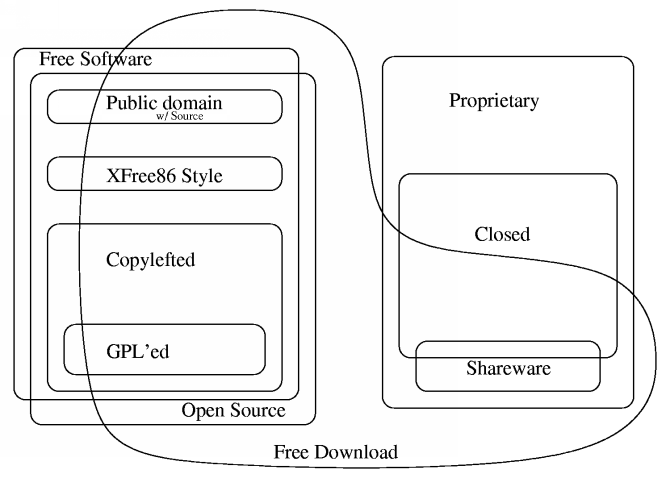
\includegraphics[width=200pt,height=170pt]{category.png}
	\end{center}

}
\subsection{Tres ejemplos concretos}
\frame
{
	\frametitle{Tres ejemplos concretos}
	\begin{itemize}
	\item MS-EULA (End User Licence Agreement
	\item Licencia GPL
	\item Licencia BSD
	\end{itemize}
}
\subsection{MS-EULA (End User Licence Agreement}
\frame
{
	\frametitle{MS-EULA (End User Licence Agreement}
	\begin{itemize}
	\item Se prohibe la copia
	\item El software solo puede ser empleado en un �nico ordenador con un m�ximo de 2 procesadores
	\item No puede ser empleado como webserver o fileserver.
	\item Puede dejar de funcionar si se efect�an cambios en el hardware.
	\item Las actualizaciones del sistema pueden modificar la EULA.
	\item Solo puede ser transferida una vez a otro usuario.
	\item Limita la ingenier�a inversa.
	\item S� podr� en cualquier momento recoger informaci�n del sistema y su uso, la cual podr� suministrar dicha informaci�n a terceros.
	\item La garant�a tan solo cubre los primeros 90 d�as.
	\item Actualizaciones y parches sin garant�a.
	\end{itemize}
}

\subsection{Licencia GPL}
\frame
{	
	\frametitle{GPL}
	\begin{itemize}
	\item Permite la copia, modificaci�n y redistribuci�n del software.
	\item Garant�a de los derechos del ciudadano a la copia, modificaci�n y redistribuci�n del software.
	\item No ofrece garant�as sobre el producto.
	\item Puede ser vendido y se puede cobrar por los servicios sobre el software.
	\item Cualquier patente sobre el mismo debe ser licenciada para el beneficio de todos.
	\item Debe incluir el c�digo fuente.
	\end{itemize}
}
\subsection{Licencia BSD}
\frame	
{
	\frametitle{BSD}
        \begin{itemize}
        \item Software Libre
        \item Cumple con las tres libertades
        \item No es copyleft como la GPL.
        \item Es posible cambiar la licencia.
        \item FreeBSD y el NetBSD.                                                                  \item Con los programas BSD, usted est� autorizado a copiarlos y distribuirlos libremente a cuantos quiera y lo podr� hacer por dinero o regal�ndolos
        \item \textbf{Desventajas}
	\end{itemize}
	
}
